\section{Vorwissen: Relaisbetrieb} \label{sec:vorwissen} \index{Relaisbetrieb}
In diesem Abschnitt werde ich kurz den \emph{klassischen} FM-Relaisbetrieb auf VHF und UHF im Amateurfunk beschreiben. Die allermeisten lizenzierten Funkamateure werde dies noch aus der Prüfung zur Betriebstechnik oder aus eigener Erfahrung wissen. 

Wenn Sie sich aber für Amateurfunk interessieren oder selbst noch keine Erfahrung mit dem Relaisbetrieb haben, empfehle ich Ihnen diesen Abschnitt zu lesen. 

\begin{figure}[!ht]
 \centering
 \documentclass{standalone}
\newcommand{\repeater}[3]{%
 \node ({#1}) at ({#2}) {%
  \begin{tikzpicture}%
   \draw [black,thick] (-.25,0) -- (0,0.5) -- (0.25,0) -- (-0.25,0);%
   \draw [black,thick,domain=-45:225] plot ({0.2*cos(\x)}, {0.5+0.2*sin(\x)});%
   \draw [black,thick,domain=-45:225] plot ({0.4*cos(\x)}, {0.5+0.4*sin(\x)});%
   \node (xxx) at (0,-.2) {{#3}};%
  \end{tikzpicture}%
 } %
}

\newcommand{\activerepeater}[3]{%
 \node ({#1}) at ({#2}) {%
  \begin{tikzpicture}%
   \draw [black,thick] (-.25,0) -- (0,0.5) -- (0.25,0) -- (-0.25,0);%
   \draw [red,thick,domain=-45:225] plot ({0.2*cos(\x)}, {0.5+0.2*sin(\x)});%
   \draw [red,thick,domain=-45:225] plot ({0.4*cos(\x)}, {0.5+0.4*sin(\x)});%
   \node (xxx) at (0,-.2) {{#3}};%
  \end{tikzpicture}%
 } %
}


\newcommand{\user}[3]{%
 \node ({#1}) at ({#2}) {%
  \begin{tikzpicture}%
   \draw [black,fill=black] (-.25,0) -- (0,0.5) -- (0.25,0) -- (-0.25,0);%
   \draw [black,fill=black] (0,.5) circle (.2); %
   \node (xxx) [text width=0.6cm, align=center] at (-.35cm,-.4) {{#3}};%
  \end{tikzpicture}%
 } %
}

\newcommand{\activeuser}[3]{%
 \node ({#1}) at ({#2}) {%
  \begin{tikzpicture}%
   \draw [red,fill=red] (-.25,0) -- (0,0.5) -- (0.25,0) -- (-0.25,0);%
   \draw [red,fill=red] (0,.5) circle (.2); %
   \node (xxx) [text width=0.6cm, align=center] at (-.35cm,-.4) {{#3}};%
  \end{tikzpicture}%
 } %
}

\begin{document}
 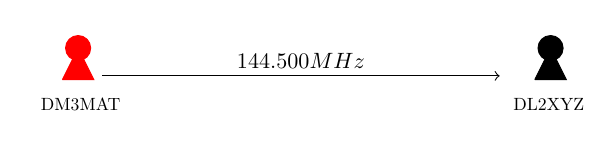
\begin{tikzpicture}[every node/.style={scale=.8}]
  \activeuser{U1}{0,0}{DM3MAT};
  \user{U2}{6,0}{DL2XYZ};
  \path[->] (U1) edge node[above] {$144.500 MHz$} (U2) ;
 \end{tikzpicture}
\end{document}

 \documentclass{standalone}
\newcommand{\repeater}[3]{%
 \node ({#1}) at ({#2}) {%
  \begin{tikzpicture}%
   \draw [black,thick] (-.25,0) -- (0,0.5) -- (0.25,0) -- (-0.25,0);%
   \draw [black,thick,domain=-45:225] plot ({0.2*cos(\x)}, {0.5+0.2*sin(\x)});%
   \draw [black,thick,domain=-45:225] plot ({0.4*cos(\x)}, {0.5+0.4*sin(\x)});%
   \node (xxx) at (0,-.2) {{#3}};%
  \end{tikzpicture}%
 } %
}

\newcommand{\activerepeater}[3]{%
 \node ({#1}) at ({#2}) {%
  \begin{tikzpicture}%
   \draw [black,thick] (-.25,0) -- (0,0.5) -- (0.25,0) -- (-0.25,0);%
   \draw [red,thick,domain=-45:225] plot ({0.2*cos(\x)}, {0.5+0.2*sin(\x)});%
   \draw [red,thick,domain=-45:225] plot ({0.4*cos(\x)}, {0.5+0.4*sin(\x)});%
   \node (xxx) at (0,-.2) {{#3}};%
  \end{tikzpicture}%
 } %
}


\newcommand{\user}[3]{%
 \node ({#1}) at ({#2}) {%
  \begin{tikzpicture}%
   \draw [black,fill=black] (-.25,0) -- (0,0.5) -- (0.25,0) -- (-0.25,0);%
   \draw [black,fill=black] (0,.5) circle (.2); %
   \node (xxx) [text width=0.6cm, align=center] at (-.35cm,-.4) {{#3}};%
  \end{tikzpicture}%
 } %
}

\newcommand{\activeuser}[3]{%
 \node ({#1}) at ({#2}) {%
  \begin{tikzpicture}%
   \draw [red,fill=red] (-.25,0) -- (0,0.5) -- (0.25,0) -- (-0.25,0);%
   \draw [red,fill=red] (0,.5) circle (.2); %
   \node (xxx) [text width=0.6cm, align=center] at (-.35cm,-.4) {{#3}};%
  \end{tikzpicture}%
 } %
}

\begin{document}
 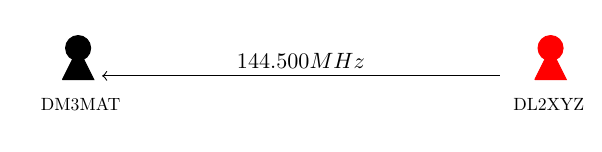
\begin{tikzpicture}[every node/.style={scale=.8}]
  \user{U1}{0,0}{DM3MAT};
  \activeuser{U2}{6,0}{DL2XYZ};
  \path[->] (U2) edge node[above] {$144.500 MHz$} (U1) ;
 \end{tikzpicture}
\end{document}

 \caption{Einfacher Simplexbetrieb, DM3MAT sendet auf der Frequenz $144.500 MHz$ direkt zu DL2XYZ. Dieser antwortet dann auf der selben Frequenz.} \label{fig:basicsimlpex}
\end{figure}

Die meisten Verbindungen zwischen zwei Funkamateuren finden im so genannten \adef{Simplexbetrieb} statt. Das heißt, die zwei Funkamateure senden und empfangen abwechselnd auf der selben Frequenz und die Verbindung zwischen ihnen ist direkt (siehe Abb. \ref{fig:basicsimlpex}). Dies funktioniert auf Kurzwelle\footnote{Als Kurzwelle oder einfach HF (\emph{high frequency}) werden Frequenzen zwischen $3MHz$ und $30MHz$ bezeichnet.} sehr gut und man kann damit weltweite Verbindungen aufbauen. 

Auf höheren Frequenzen verhält sich die Radiowelle zunehmend wie Licht und es wird auf VHF\footnote{Als VHF (\emph{very high frequency}) werden die Frequenzen zwischen $30Mhz$ und $300MHz$ bezeichnet.} und UHF\footnote{Als UHF (\emph{ultra high frequency}) werden die Frequenzen zwischen $300Mhz$ und $3000MHz$ bezeichnet.} schwierig ohne viel Aufwand\footnote{Auch auf VHF und UHF können sehr große Entfernungen überbrückt werden, nur sind dann große Richtantennen oder ein sehr hoher Standort von Nöten.} wesentlich weiter als bis zum Horizont zu gelangen. Diese Tatsache schränkt die Reichweite gerade von Handfunkgeräten stark ein. Um dennoch einen größeren Bereich überbrücken zu können, wenn man nicht gerade über einen hohen Berg mit einer großen Antenne verfügt, können sogenannte Repeater oder Relais verwendet werden. 

\adef{Repeater}\index{Relais|seealso{Repeater}} sind automatisch arbeitende Amateurfunkstationen, die meist in exponierten Lagen (hoher Berg oder hoher Turm) installiert werden, um einen möglichst großen Bereich abdecken zu können. Ihre Aufgabe ist es, Aussendungen von Funkamateuren zu empfangen und gleichzeitig wieder auszusenden. Da diese Repeater gleichzeitig empfangen und senden müssen, können sie das nicht auf der selben Frequenz tun. Daher werden diese Repeater im sogenannten \adef{Duplexbetrieb} gefahren. Das heißt, der Repeater empfängt auf einer Frequenz (der sog. \adef{Eingabefrequenz}) und sendet eben dieses empfangende Signal gleichzeitig auf einer anderen Frequenz (der sog. \adef{Ausgabefrequenz}) wieder aus. 

\begin{figure}[!ht]
 \centering
 \documentclass{standalone}
\usepackage{tikz}
\usetikzlibrary{shapes.geometric}
\newcommand{\repeater}[3]{%
 \node ({#1}) at ({#2}) {%
  \begin{tikzpicture}%
   \draw [black,thick] (-.25,0) -- (0,0.5) -- (0.25,0) -- (-0.25,0);%
   \draw [black,thick,domain=-45:225] plot ({0.2*cos(\x)}, {0.5+0.2*sin(\x)});%
   \draw [black,thick,domain=-45:225] plot ({0.4*cos(\x)}, {0.5+0.4*sin(\x)});%
   \node (xxx) at (0,-.2) {{#3}};%
  \end{tikzpicture}%
 } %
}

\newcommand{\activerepeater}[3]{%
 \node ({#1}) at ({#2}) {%
  \begin{tikzpicture}%
   \draw [black,thick] (-.25,0) -- (0,0.5) -- (0.25,0) -- (-0.25,0);%
   \draw [red,thick,domain=-45:225] plot ({0.2*cos(\x)}, {0.5+0.2*sin(\x)});%
   \draw [red,thick,domain=-45:225] plot ({0.4*cos(\x)}, {0.5+0.4*sin(\x)});%
   \node (xxx) at (0,-.2) {{#3}};%
  \end{tikzpicture}%
 } %
}


\newcommand{\user}[3]{%
 \node ({#1}) at ({#2}) {%
  \begin{tikzpicture}%
   \draw [black,fill=black] (-.25,0) -- (0,0.5) -- (0.25,0) -- (-0.25,0);%
   \draw [black,fill=black] (0,.5) circle (.2); %
   \node (xxx) [text width=0.6cm, align=center] at (-.35cm,-.4) {{#3}};%
  \end{tikzpicture}%
 } %
}

\newcommand{\activeuser}[3]{%
 \node ({#1}) at ({#2}) {%
  \begin{tikzpicture}%
   \draw [red,fill=red] (-.25,0) -- (0,0.5) -- (0.25,0) -- (-0.25,0);%
   \draw [red,fill=red] (0,.5) circle (.2); %
   \node (xxx) [text width=0.6cm, align=center] at (-.35cm,-.4) {{#3}};%
  \end{tikzpicture}%
 } %
}

\begin{document}
 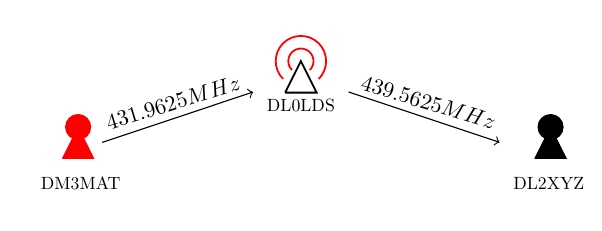
\begin{tikzpicture}[every node/.style={scale=.8}]
  \activeuser{U1}{0,0}{DM3MAT};
  \activerepeater{R1}{3,1}{DL0LDS};
  \user{U2}{6,0}{DL2XYZ};
  \path[->] (U1) edge node[above,rotate=17] {$431.9625 MHz$} (R1) ;
  \path[->] (R1) edge node[above,rotate=-17] {$439.5625 MHz$} (U2);
 \end{tikzpicture}
\end{document}

 \documentclass{standalone}
\newcommand{\repeater}[3]{%
 \node ({#1}) at ({#2}) {%
  \begin{tikzpicture}%
   \draw [black,thick] (-.25,0) -- (0,0.5) -- (0.25,0) -- (-0.25,0);%
   \draw [black,thick,domain=-45:225] plot ({0.2*cos(\x)}, {0.5+0.2*sin(\x)});%
   \draw [black,thick,domain=-45:225] plot ({0.4*cos(\x)}, {0.5+0.4*sin(\x)});%
   \node (xxx) at (0,-.2) {{#3}};%
  \end{tikzpicture}%
 } %
}

\newcommand{\activerepeater}[3]{%
 \node ({#1}) at ({#2}) {%
  \begin{tikzpicture}%
   \draw [black,thick] (-.25,0) -- (0,0.5) -- (0.25,0) -- (-0.25,0);%
   \draw [red,thick,domain=-45:225] plot ({0.2*cos(\x)}, {0.5+0.2*sin(\x)});%
   \draw [red,thick,domain=-45:225] plot ({0.4*cos(\x)}, {0.5+0.4*sin(\x)});%
   \node (xxx) at (0,-.2) {{#3}};%
  \end{tikzpicture}%
 } %
}


\newcommand{\user}[3]{%
 \node ({#1}) at ({#2}) {%
  \begin{tikzpicture}%
   \draw [black,fill=black] (-.25,0) -- (0,0.5) -- (0.25,0) -- (-0.25,0);%
   \draw [black,fill=black] (0,.5) circle (.2); %
   \node (xxx) [text width=0.6cm, align=center] at (-.35cm,-.4) {{#3}};%
  \end{tikzpicture}%
 } %
}

\newcommand{\activeuser}[3]{%
 \node ({#1}) at ({#2}) {%
  \begin{tikzpicture}%
   \draw [red,fill=red] (-.25,0) -- (0,0.5) -- (0.25,0) -- (-0.25,0);%
   \draw [red,fill=red] (0,.5) circle (.2); %
   \node (xxx) [text width=0.6cm, align=center] at (-.35cm,-.4) {{#3}};%
  \end{tikzpicture}%
 } %
}

\begin{document}
 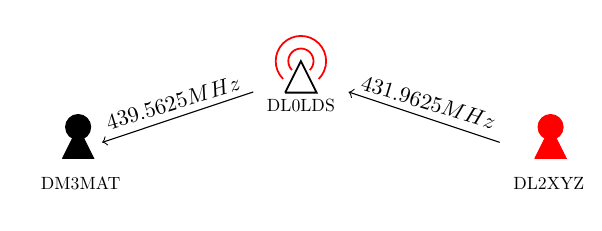
\begin{tikzpicture}[every node/.style={scale=.8}]
  \user{U1}{0,0}{DM3MAT};
  \activerepeater{R1}{3,1}{DL0LDS};
  \activeuser{U2}{6,0}{DL2XYZ};
  \path[->] (U2) edge node[above,rotate=-17] {$431.9625 MHz$} (R1) ;
  \path[->] (R1) edge node[above,rotate=17] {$439.5625 MHz$} (U1);
 \end{tikzpicture}
\end{document}

 \caption{Einfacher Repeaterbetrieb, DM3MAT sendet auf der Eingabefrequenz $431.9625 MHz$ zum Repeater (DB0LDS) und dieser setzt das empfangende Signal direct auf der Ausgabefrequenz $439.5625 MHz$ wieder ab. Auf dieser Frequenz kann DL2XYZ das umgesetzte Signal wieder empfangen.} \label{fig:basicrepeater}
\end{figure}

Für das konkrete Beispiel in Abbildung \ref{fig:basicrepeater} bedeutet das, dass DM3MAT auf der Repeatereingabefrequenz (hier $431.9625 MHz$) sendet. Dieses Signal wird vom Repeater (hier DB0LDS) empfangen und gleichzeitig wieder auf der Ausgabefrequenz (hier $439.5625 MHz$) ausgesandt. Diese Aussendung kann nun von DL2XYZ auf der Repeaterausgabefrequenz empfangen werden. Die Antwort von DL2XYZ an DM3MAT folgt den gleichen Weg, hier sendet DL2XYZ auf der Repeatereingabefrequenz und DM3MAT kann diese Aussendung auf der Repeaterausgabefrequenz empfangenen. Auf diese Wiese können zwei Funkamateure miteinander kommunizieren, auch wenn sie sich nicht direkt erreichen können. 

\subsection{Echolink} \label{sec:echolink} \index{Echolink}
Wenn zwei Funkamateure miteinander kommunizieren wollen, die sehr weit voneinander entfernt sind und somit nicht beide einen gemeinsamen Repeater erreichen können, gibt es die Möglichkeit zwei Repeater \emph{zusammenzuschalten}. 

\begin{figure}[!ht]
 \centering
 \documentclass{standalone}
\newcommand{\repeater}[3]{%
 \node ({#1}) at ({#2}) {%
  \begin{tikzpicture}%
   \draw [black,thick] (-.25,0) -- (0,0.5) -- (0.25,0) -- (-0.25,0);%
   \draw [black,thick,domain=-45:225] plot ({0.2*cos(\x)}, {0.5+0.2*sin(\x)});%
   \draw [black,thick,domain=-45:225] plot ({0.4*cos(\x)}, {0.5+0.4*sin(\x)});%
   \node (xxx) at (0,-.2) {{#3}};%
  \end{tikzpicture}%
 } %
}

\newcommand{\activerepeater}[3]{%
 \node ({#1}) at ({#2}) {%
  \begin{tikzpicture}%
   \draw [black,thick] (-.25,0) -- (0,0.5) -- (0.25,0) -- (-0.25,0);%
   \draw [red,thick,domain=-45:225] plot ({0.2*cos(\x)}, {0.5+0.2*sin(\x)});%
   \draw [red,thick,domain=-45:225] plot ({0.4*cos(\x)}, {0.5+0.4*sin(\x)});%
   \node (xxx) at (0,-.2) {{#3}};%
  \end{tikzpicture}%
 } %
}


\newcommand{\user}[3]{%
 \node ({#1}) at ({#2}) {%
  \begin{tikzpicture}%
   \draw [black,fill=black] (-.25,0) -- (0,0.5) -- (0.25,0) -- (-0.25,0);%
   \draw [black,fill=black] (0,.5) circle (.2); %
   \node (xxx) [text width=0.6cm, align=center] at (-.35cm,-.4) {{#3}};%
  \end{tikzpicture}%
 } %
}

\newcommand{\activeuser}[3]{%
 \node ({#1}) at ({#2}) {%
  \begin{tikzpicture}%
   \draw [red,fill=red] (-.25,0) -- (0,0.5) -- (0.25,0) -- (-0.25,0);%
   \draw [red,fill=red] (0,.5) circle (.2); %
   \node (xxx) [text width=0.6cm, align=center] at (-.35cm,-.4) {{#3}};%
  \end{tikzpicture}%
 } %
}

\begin{document}
 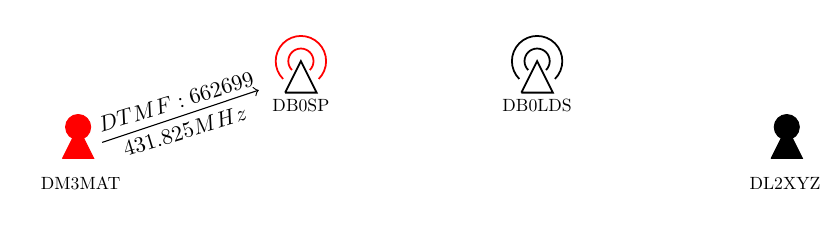
\begin{tikzpicture}[every node/.style={scale=.8}]
  \activeuser{U1}{0,0}{DM3MAT};
  \activerepeater{R1}{3,1}{DB0SP};
  \repeater{R2}{6,1}{DB0LDS};
  \user{U2}{9,0}{DL2XYZ};
  \path[->] (U1) edge node[above,rotate=17] {$DTMF: 662699$} node[below,rotate=17]{$431.825 MHz$} (R1) ;
 \end{tikzpicture}
\end{document}

 \documentclass{standalone}
\newcommand{\repeater}[3]{%
 \node ({#1}) at ({#2}) {%
  \begin{tikzpicture}%
   \draw [black,thick] (-.25,0) -- (0,0.5) -- (0.25,0) -- (-0.25,0);%
   \draw [black,thick,domain=-45:225] plot ({0.2*cos(\x)}, {0.5+0.2*sin(\x)});%
   \draw [black,thick,domain=-45:225] plot ({0.4*cos(\x)}, {0.5+0.4*sin(\x)});%
   \node (xxx) at (0,-.2) {{#3}};%
  \end{tikzpicture}%
 } %
}

\newcommand{\activerepeater}[3]{%
 \node ({#1}) at ({#2}) {%
  \begin{tikzpicture}%
   \draw [black,thick] (-.25,0) -- (0,0.5) -- (0.25,0) -- (-0.25,0);%
   \draw [red,thick,domain=-45:225] plot ({0.2*cos(\x)}, {0.5+0.2*sin(\x)});%
   \draw [red,thick,domain=-45:225] plot ({0.4*cos(\x)}, {0.5+0.4*sin(\x)});%
   \node (xxx) at (0,-.2) {{#3}};%
  \end{tikzpicture}%
 } %
}


\newcommand{\user}[3]{%
 \node ({#1}) at ({#2}) {%
  \begin{tikzpicture}%
   \draw [black,fill=black] (-.25,0) -- (0,0.5) -- (0.25,0) -- (-0.25,0);%
   \draw [black,fill=black] (0,.5) circle (.2); %
   \node (xxx) [text width=0.6cm, align=center] at (-.35cm,-.4) {{#3}};%
  \end{tikzpicture}%
 } %
}

\newcommand{\activeuser}[3]{%
 \node ({#1}) at ({#2}) {%
  \begin{tikzpicture}%
   \draw [red,fill=red] (-.25,0) -- (0,0.5) -- (0.25,0) -- (-0.25,0);%
   \draw [red,fill=red] (0,.5) circle (.2); %
   \node (xxx) [text width=0.6cm, align=center] at (-.35cm,-.4) {{#3}};%
  \end{tikzpicture}%
 } %
}

\begin{document}
 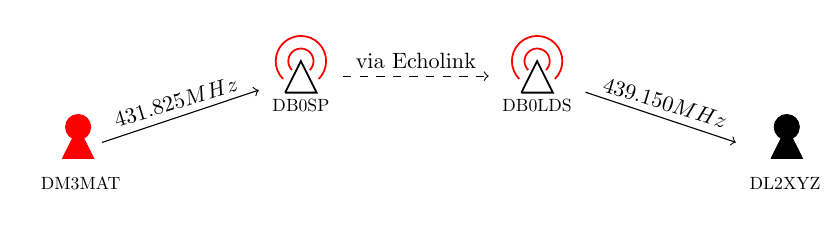
\begin{tikzpicture}[every node/.style={scale=.8}]
  \activeuser{U1}{0,0}{DM3MAT};
  \activerepeater{R1}{3,1}{DB0SP};
  \activerepeater{R2}{6,1}{DB0LDS};
  \user{U2}{9,0}{DL2XYZ};
  \path[->] (U1) edge node[above,rotate=17] {$431.825 MHz$} (R1) ;
  \path[->,dashed] (R1) edge node[above] {via Echolink} (R2) ;	
  \path[->] (R2) edge node[above,rotate=-17] {$439.150 MHz$} (U2) ;
 \end{tikzpicture}
\end{document}

 \documentclass{standalone}
\usepackage{tikz}
\usetikzlibrary{shapes.geometric}
\newcommand{\repeater}[3]{%
 \node ({#1}) at ({#2}) {%
  \begin{tikzpicture}%
   \draw [black,thick] (-.25,0) -- (0,0.5) -- (0.25,0) -- (-0.25,0);%
   \draw [black,thick,domain=-45:225] plot ({0.2*cos(\x)}, {0.5+0.2*sin(\x)});%
   \draw [black,thick,domain=-45:225] plot ({0.4*cos(\x)}, {0.5+0.4*sin(\x)});%
   \node (xxx) at (0,-.2) {{#3}};%
  \end{tikzpicture}%
 } %
}

\newcommand{\activerepeater}[3]{%
 \node ({#1}) at ({#2}) {%
  \begin{tikzpicture}%
   \draw [black,thick] (-.25,0) -- (0,0.5) -- (0.25,0) -- (-0.25,0);%
   \draw [red,thick,domain=-45:225] plot ({0.2*cos(\x)}, {0.5+0.2*sin(\x)});%
   \draw [red,thick,domain=-45:225] plot ({0.4*cos(\x)}, {0.5+0.4*sin(\x)});%
   \node (xxx) at (0,-.2) {{#3}};%
  \end{tikzpicture}%
 } %
}


\newcommand{\user}[3]{%
 \node ({#1}) at ({#2}) {%
  \begin{tikzpicture}%
   \draw [black,fill=black] (-.25,0) -- (0,0.5) -- (0.25,0) -- (-0.25,0);%
   \draw [black,fill=black] (0,.5) circle (.2); %
   \node (xxx) [text width=0.6cm, align=center] at (-.35cm,-.4) {{#3}};%
  \end{tikzpicture}%
 } %
}

\newcommand{\activeuser}[3]{%
 \node ({#1}) at ({#2}) {%
  \begin{tikzpicture}%
   \draw [red,fill=red] (-.25,0) -- (0,0.5) -- (0.25,0) -- (-0.25,0);%
   \draw [red,fill=red] (0,.5) circle (.2); %
   \node (xxx) [text width=0.6cm, align=center] at (-.35cm,-.4) {{#3}};%
  \end{tikzpicture}%
 } %
}

\begin{document}
 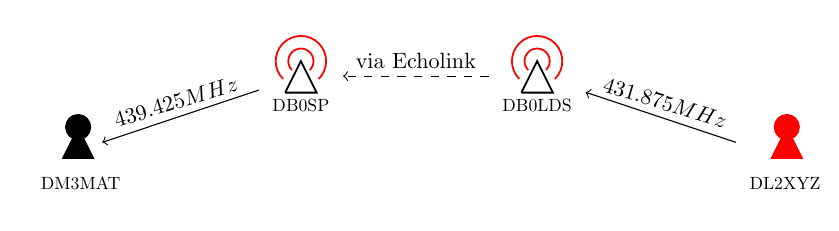
\begin{tikzpicture}[every node/.style={scale=.8}]
  \user{U1}{0,0}{DM3MAT};
  \activerepeater{R1}{3,1}{DB0SP};
  \activerepeater{R2}{6,1}{DB0LDS};
  \activeuser{U2}{9,0}{DL2XYZ};
  \path[->] (R1) edge node[above,rotate=17] {$439.425 MHz$} (U1) ;
  \path[->,dashed] (R2) edge node[above] {via Echolink} (R1) ;	
  \path[->] (U2) edge node[above,rotate=-17] {$431.875 MHz$} (R2) ;
 \end{tikzpicture}
\end{document}

 \caption{Repeaterbetrieb mit Echolink. DM3MAT verbindet die Repeater DB0SP (bei Berlin) und DB0LEI (bei Leipzig) per Echolink. Daraufhin können DM3MAT und DL2XYZ wie über einen gemeinsamen Repeater kommunizieren.} \label{fig:echolink}
\end{figure}

Diese Möglichkeit nennt sich \href{http://www.echolink.org/}{Echolink}. Dieses Netzwerk erlaubt es FM Repeater per Internet miteinander zu verbinden oder sich per Internet als einzelner Teilnehmer direkt mit einem Repeater zu verbinden. Viele FM Repeater sind in diesem Netzwerk zusammengeschlossen. 

Es ist auch häufig möglich\footnote{Dies hängt von der Konfiguration des Repeaters ab.} per Funk einen Repeater zu steuern und ihn mit einem anderen Repeater via Echolink zu verbinden. Dazu wird die sogenannte Echolink Nummer des Ziel Repeaters per DTMF Tonwahl an den Quellrepeater gesandt. Dies ist in Abbildung \ref{fig:echolink} (Oben) dargestellt. Hier sendet DM3MAT die Echolink Nummer 662699 des Relais DB0LEI bei Leipzig per DTMF an den Repeater DB0SP nahe Berlin. Dieser (DB0SP) verbindet sich dann mit dem Zielrepeater bei Leipzig (DB0LEI) über das Echolink Netzwerk. Alle weiteren Aussendungen die der Quellrepeater (DB0SP) nun empfängt werden nicht nur lokal auf der Ausgabefrequenz ausgesandt, sonder werden auch am Zielrepeater bei Leipzig (DB0LEI) ausgesandt (Abb. \ref{fig:echolink} Mitte). Somit kann DL2XYZ in Leipzig DM3MAT hören. Ebenso werden alle Aussendungen die der Zielrepeater (DB0LEI) empfängt via Echolink zum Quellrepeater bei Berlin übertragen und auch dort ausgesandt (Abb. \ref{fig:echolink} Unten).  Auf diese weise können zwei Funkamateure (in diesem Beispiel DM3MAT \& DL2XYZ), die sich nicht in der Nähe des selben Repeaters befinden, dennoch miteinander kommunizieren. 

\begin{merke}
Sobald zwei Repeater per Echolink miteinander verbunden sind, verhalten sich beide wie ein einziger Repeater. 
\end{merke}

Es gibt überall auf der Welt FM Repeater die per Echolink erreichbar sind. Dadurch ist es möglich jederzeit weltweite Kontakte mit einfachsten Mitteln (FM Handfunkgeräte mit DTMF Funktion sind ab ca. \EUR{40} erhältlich) herzustellen.